%!TEX root = ./template-skripsi.tex
%-------------------------------------------------------------------------------
%                            BAB II
%               KAJIAN TEORI
%-------------------------------------------------------------------------------

\chapter{KAJIAN PUSTAKA}                


\section{Pengolahan Citra Digital (\emph{Digital Image Processing})}
Citra dapat didefinisikan sebagai fungsi dua dimensi $f(x,y)$ di mana $x$ dan $y$ adalah koordinat bidang, dan $f$ pada pasangan koordinat $(x,y)$ disebut intensitas(\emph{intensity}) atau tingkat abu-abu(\emph{gray-level}) citra pada saat itu. Jika $x$, $y$, dan nilai intensitas $f$ semuanya terbatas, dan dapat ditentukan nilainya secara diskrit, maka citra tersebut kita sebut sebagai citra digital(\emph{digital image}). Citra digital direpresentasikan sebagai matriks berukuran $M$ x $N$ yang menyatakan resolusi citra, dan setiap elemen matriks menyatakan sebuah pixel(\emph{picture element})
\begin{figure}[H]
	\centering
	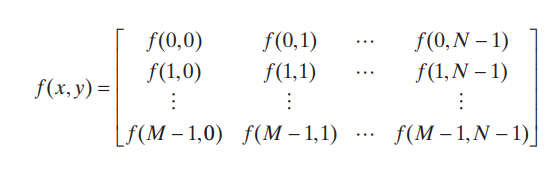
\includegraphics[width=1\textwidth]{gambar/digitalimage}
	\caption{Representasi Citra Digital}
	\label{Gambar:digitalimage}
\end{figure}
Bidang pengolahan citra digital mengacu pada pengolahan citra digital dengan menggunakan komputer digital. Perhatikan bahwa citra digital terdiri dari sejumlah elemen yang terbatas, yang masing-masing memiliki lokasi dan nilai tertentu. Salah satu kelebihan citra digital adalah kemudahan dalam melakukan pengolahan atau manipulasi citra, untuk melakukan hal tersebut diperlukan proses yang dikenal sebagai pengolahan citra(\emph{image processing})\citep{gonzalez2002digital}.
\subsection{Citra \emph{Grayscale}}
Dalam operasi pengolahan citra, sebagian besar operasi dilakukan dalam gambar \emph{grayscale}\citep{tyagi2018understanding}. Citra \emph{grayscale} adalah citra yang hanya memiliki satu kanal pada setiap pixel nya yang mewakili intensitas. Intensitas piksel berada dalam kisaran [0, 255] yang mana hal ini menunjukkan tingkat terangnya atau tingkat cahaya dari suatu pixel. Warna pada citra \emph{grayscale} merupakan warna abu dengan tingkatan dari hitam hingga sampai putih(tingkat keabuan). Kisaran intensitas piksel bernilai 0 artinya hitam dan 255 adalah putih(untuk \emph{256-graylevel}).
\begin{figure}[H]
	\centering
	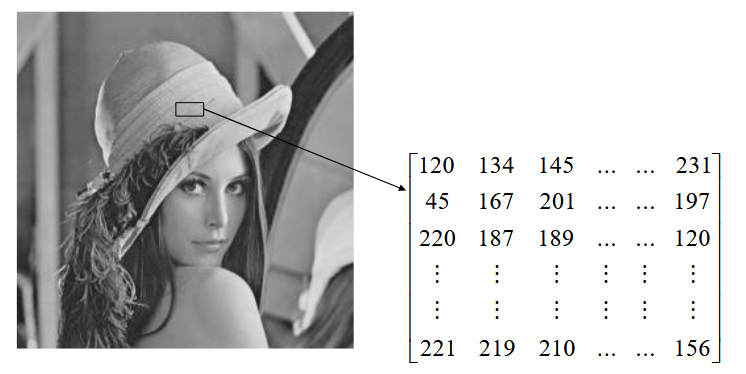
\includegraphics[width=1\textwidth]{gambar/grayimage}
	\caption{Contoh citra \emph{grayscale}}
	\label{Gambar:grayimage}
\end{figure}

Setiap piksel dalam gambar umumnya dijelaksan oleh kombinasi tiga nilai intensitas R(\emph{red}), G(\emph{green}),dan B(\emph{blue}). Salah satu cara memetakan nilai tersebut ke satu nilai \emph{grayscale} adalah dengan menggunakan metode \emph{luminosity}\citep{kumar2016gray}.
\begin{equation}
	\label{luminosity}
	L = 0.21 R + 0.72 G + 0.07 B.
\end{equation}

\begin{figure}[H]
	\centering
	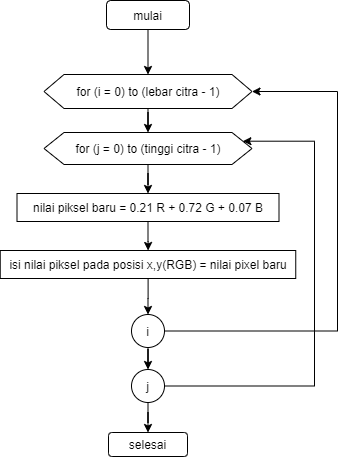
\includegraphics[width=0.6\textwidth]{diagram/grayscale}
	\caption{Proses konversi citra RGB menjadi \emph{grayscale}}
	\label{Gambar:grayscalediagram}
\end{figure}

\section{\emph{Gaussian Filter/Gaussian Blur}}
Peningkatan kualitas citra(\emph{image enhancement}) adalah proses mengedit gambar untuk membuatnya 'lebih baik' untuk aplikasi tertentu\citep{tyagi2018understanding}. Hal ini melibatkan proses menghaluskan atau mempertajam konten gambar. Salah satu metode dalam proses menghaluskan gambar adalah \emph{filtering}, salah satunya adalah dengan menggunakan metode \emph{Gaussian filter/Gaussian Blur}. Proses ini adalah proses memblur gambar menggunakan fungsi gaussian dengan tujuan mengurangi \emph{noise} gambar dan mengurangi detail tertentu. \emph{Gaussian blur} dideskripsikan sebagai berikut:
\begin{equation}
	\label{gaussblur}
	G(x,y) = {\frac{1}{2 \pi \sigma^2} e}^{-{\frac{x^2+y^2}{2 \sigma^2}}}
\end{equation}
Pengaruh filter \emph{gaussian blur} dengan berbagai standar deviasi $\sigma$ ditunjukkan pada Gambar berikut:
\begin{figure}[H]
	\centering
	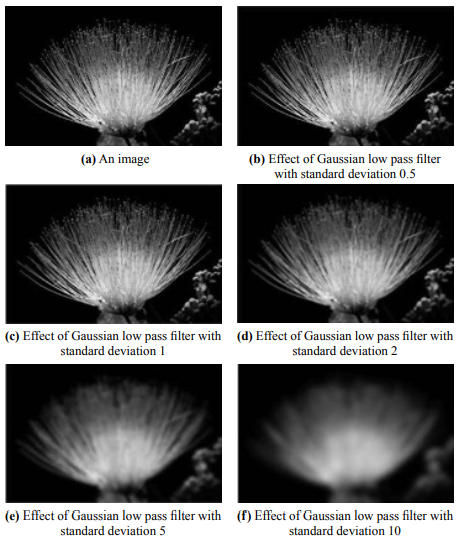
\includegraphics[width=1\textwidth]{gambar/gaussianfilter}
	\caption{Gambar dan efek \emph{gaussian blur} dengan berbagai standar deviasi\citep{tyagi2018understanding}}
	\label{Gambar:gaussianfilter}
\end{figure}

\section{Kurva parametrik(\emph{parametric curve})}
Untuk mempelajari model \emph{snake} dasar yang diperkenalkan oleh Kass et. al., kita perlu memahami tentang kurva parametrik. Kurva parametrik adalah kurva kontinu pada bidang dua dimensi yang dapat ditentukan oleh koordinat $x$ dan $y$, di mana nilai koordinat ini adalah fungsi kontinu dari parameter skalar, misalnya $s$. Jadi, kita dapat mengatakan bahwa $(X(s), Y(s))$ mewakili kurva kontinu dua dimensi di mana $X(s)$ dan $Y(s)$ adalah dua fungsi kontinu dari $s$ yang masing-masing mewakili koordinat $x$ dan $y$. Parameter skalar $s$ yang sering diperbolehkan antara $0$ dan $1$, dengan kata lain, $s \in [0, 1]$. Kasus yang sering terjadi ketika menggunakan model \emph{snake} ini adalah inisialisasi kurvanya berupa kurva tertutup dimana $(X(0), Y(0))$ mewakili salah satu ujung kurva dan $(X(1), Y(1))$ ujung lainnya\citep{acton2007biomedical:19}.

Salah satu contoh kurva parametrik tertutup adalah sebuah lingkaran (bidang 2 dimensi) yang di definisikan sebagai $(X(0), Y(0))$ dan $(X(1), Y(1))$ sebagai titik yang sama, yaitu, $X(0) = X(1)$ dan $Y(0) = Y(1))$. Sebagai contoh, $X (s) = cos (2 \pi s)$ dan $Y (s) = sin (2 \pi s)$,  $s \in [0, 1] $ mendefinisikan kurva lingkaran\cite{acton2007biomedical:19}.
\begin{figure}[H]
	\centering
	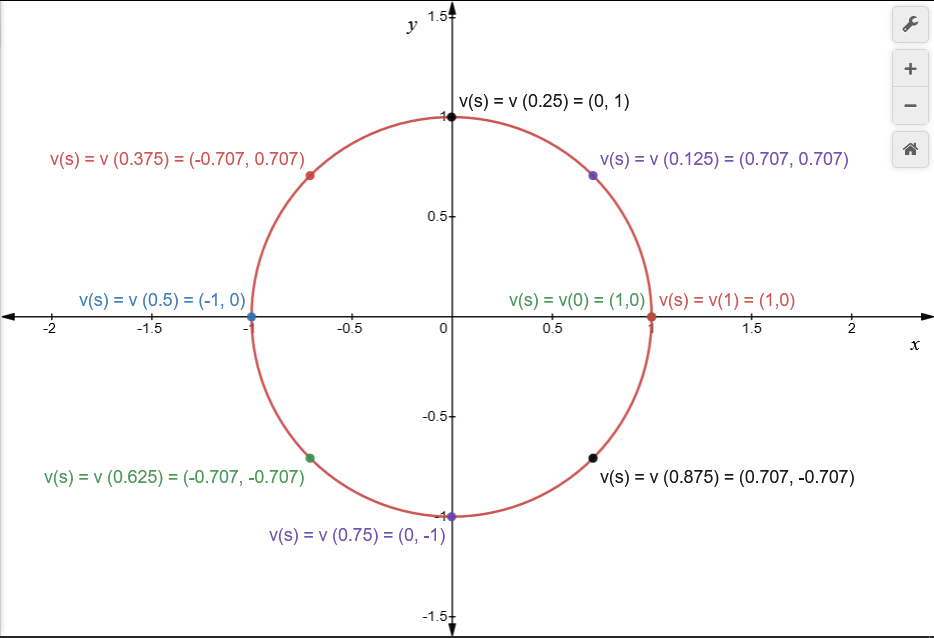
\includegraphics[width=0.4\textwidth]{gambar/k_lingkaran}
	\caption{Kurva ingkaran}
	\label{Gambar:k_lingkaran}
\end{figure}


\section{\emph{Parametric active contour}}
\emph{Parametric active contour} yang juga dikenal dengan \emph{snakes} adalah kurva yang dapat bergerak di dalam citra dari \emph{initial state} menuju ke \emph{outline} dari sebuah citra, dengan memanfaatkan \emph{functional energy} yang disebut energi internal dan energi eksternal. \emph{Snakes} di representasikan sebagai kurva $v(s) = [x(s), y(s)], s \in [0,1]$, dimana $s$ adalah panjang kurva\citep{abdullah2016robust}.
\begin{figure}[H]
	\centering
	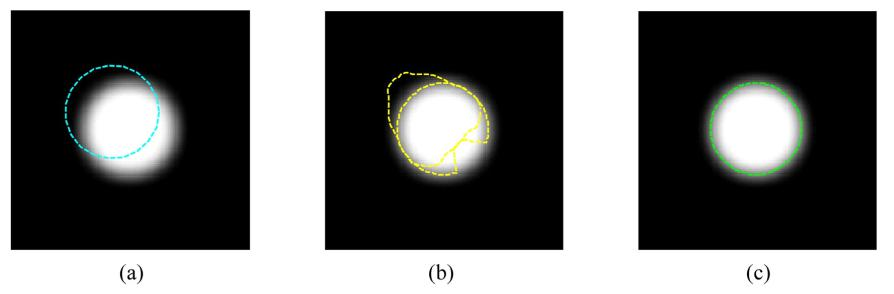
\includegraphics[width=1\textwidth]{gambar/snake1}
	\caption{(a) citra objek lingkaran \& \emph{initial snake}, (b) \emph{snake evolution},
		(c) bentuk akhir dari \emph{snake} setelah iterasi selesai \citep{acton2007biomedical:19}}
	\label{Gambar:snake1}
\end{figure}

\emph{Functional energy snake} didefinisikan sebagai berikut:
\begin{equation}
\label{eq_1}
E_{snake} = \int^1_0 E_{int}(v(s)) + \int^1_0 E_{ext}(v(s)) ds.
\end{equation}
Istilah $E_{int}(v(s))$ dan $E_{ext}(v(s))$ masing-masing adalah energi internal dan eksternal \emph{snake}. Energi internal digunakan untuk mengontrol deformabilitas \emph{snake}, yang dapat ditulis sebagai berikut:
\begin{equation}
\label{eq_2}
E_{int}(v(s)) = \frac{1}{2} \left(\alpha(s)|v_{s}(s)|^2 + \beta(s)|v_{ss}(s)|^2\right)
\end{equation}
dimana $v_{s}$ adalah turunan pertama yang merepresentasikan \emph{elasticity}, sedangkan $v_{ss}$ adalah turunan kedua dan merepresentasikan \emph{rigidity}, koefisien $\alpha$ dan $\beta$ adalah parameter yang mengontrol hal tersebut\citep{abdullah2016robust}.

Fungsi energi eksternal diturunkan dari energi diluar kurva, yang berarti dari citra itu sendiri. Sebagai salah satu opsi, energi eksternal dapat didefinisikan sebagai berikut:
\begin{equation}
\label{eq_3}
E_{ext} (v(s)) = -|\nabla (  G_{\sigma}(x,y) \ast I(x,y) ) |^2,
\end{equation}
dimana $G_{\sigma}(x,y)$ adalah fungsi \emph{Gaussian} dengan standar deviasi $\sigma$, $\nabla$ adalah operator gradien, dan $\ast$ mewakili konvolusi sedangkan $I(x,y)$ adalah fungsi intensitas gambar. Konvolusi ini memperhalus citra untuk menghilangkan \emph{noise} \citep{abdullah2016robust}.

Substitusi (\ref{eq_2}) dan (\ref{eq_3}) di (\ref{eq_1}), menghasilkan persamaan energi snake menjadi:
\begin{multline}
\label{eq_4}
E_{snake} = \int^{}_{s} \biggl(
			\frac{1}{2} \left(\alpha(s)|v_{s}(s)|^2 + \beta(s)|v_{ss}(s)|^2\right) \\
			-|\nabla (  G_{\sigma}(x,y) \ast I(x,y) ) |^2  \biggr)ds.
\end{multline}

\section{\emph{Active contour evolution}}
Untuk perhitungan evolusi Kontur aktif, kita perlu meminimalkan persamaan energi (\ref{eq_4}). Namun, perhatikan bahwa Persamaan (\ref{eq_4}) adalah fungsional, yaitu fungsi dari suatu fungsi. Untuk kasus ini, diperlukan alat pengoptimalan lanjutan dari analisis fungsional, yang dikenal sebagai kalkulus variasi atau \emph{variational calculus}. Salah satu metode turunan dari kalkulus variasi adalah persamaan Euler-Lagrange\citep{acton2007biomedical:19}.	
\subsection{Persamaan Euler-Lagrange}
Persamaan Euler-Lagrange memberi tahu kita cara mengambil turunan sehubungan dengan suatu fungsi. Setelah turunan fungsional didapatkan, selanjutnya adalah mengikuti prosedur kalkulus SMA yaitu menyamakan turunannya dengan nol dan menyelesaikan persamaan untuk mencari minimumnya. Turunan fungsional dari fungsional energi \emph{snake} (\ref{eq_4}) yang disamakan dengan nol adalah sebagai berikut\citep{acton2007biomedical:19}:
\begin{equation}
\label{eq_5}
\frac{\delta E}{\delta X} = -\alpha \frac{d^2 X}{ds^2} + \beta \frac{d^4 X}{ds^4} - \frac{\partial f}{\partial x} = 0
\end{equation}
dan
\begin{equation}
\label{eq_6}
\frac{\delta E}{\delta Y} = -\alpha \frac{d^2 Y}{ds^2} + \beta \frac{d^4 X}{ds^4} - \frac{\partial f}{\partial y} = 0
\end{equation}
Solusi dari Persamaan (\ref{eq_5}) dan (\ref{eq_6}) tidak dapat diperoleh secara umum. Salah satu metode untuk menyelesaikan Persamaan (\ref{eq_5}) dan (\ref{eq_6}) adalah menggunakan teknik numerik yang disebut metode penurunan gradien(\emph{gradient descent}).

\subsection{\emph{Gradient descent}}
Berikut contoh sederhana untuk menjelaskan prosedur \emph{gradient descent}:
\begin{figure}[H]
	\centering
	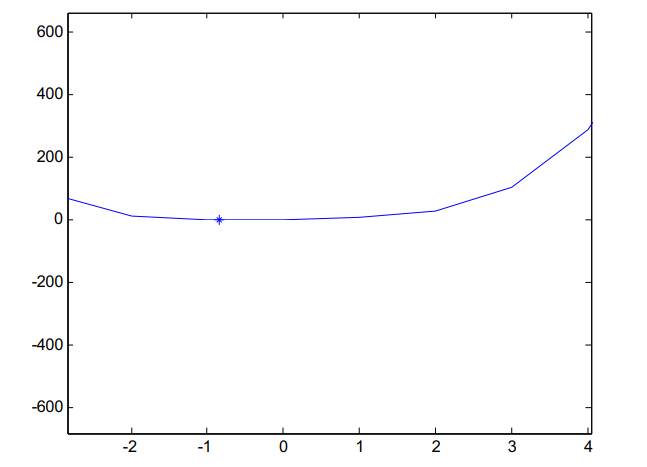
\includegraphics[width=1\textwidth]{gambar/GD1}
	\caption{Fungsi $h(x) = x^4 + x^2 + 4x + 1$ diplot dalam rentang $x$ $-3$ hingga $4$. Titik minimum adalah $-0,8351$ yang ditunjukkan dengan tanda *\citep{acton2007biomedical:19}.}
	\label{Gambar:gd1}
\end{figure}
Gambar \ref{Gambar:gd1} menunjukkan fungsi $h(x) = x^4 + x^2 + 4x + 1$. Kita ingin mencari nilai $x$ di mana $h (x)$ adalah minimum. Misalkan sebut nilai $x$ ini sebagai $x^*$. Dari pelajaran kalkulus SMA, kita tahu bahwa $x^*$ adalah solusi dari persamaan: $\frac{dh(x)}{dx} = 4x^3 + 2x + 4 = 0$. Pada beberapa kasus mungkin kita sulit mencari mencari nilai $x^*$. Dengan prinsip \emph{gradient descent}, kita mulai dengan nilai solusi tebakan awal, katakanlah $x = 0$. Kemudian, kita mengubah nilai variabel $x$ secara berulang, sehingga mendekati $x^*$ secara bertahap.

Aturan \emph{gradient descent} mengatakan bahwa perubahan $x$ harus sebanding dengan negatif dari turunan $h(x)$. Secara intuitif, ini masuk akal, setelah kita melihat Gambar \ref{Gambar:gd1}. Misalnya, pada $x = 0$, nilai turunan $\frac{dh (x = 0)}{dx}$ positif, jadi kita harus menurunkan nilai $x$ saat ini yaitu $0$ dalam kasus ini. Untuk mencapai titik minimum $x^*$, maka diterapkan aturan \emph{gradient desccent} berulang kali. Contoh lain, jika kita berada di $x = -1$, maka $\frac{dh (x = -1)}{dx}$ menjadi negatif. Secara matematis, aturan \emph{gradient descent} ini dapat dikatakan sebagai $\frac{dx}{d\tau} = - \frac{dh(x)}{dx}$, di mana $\tau$ menunjukkan variabel waktu. Dengan kata lain, perubahan sesaat dalam variabel $x$ sama dengan negatif dari turunan fungsi $h$. Paragraf ini menjelaskan bahwa untuk menyelesaikan persamaan $\frac{dh (x)}{dx}= 0$, seseorang dapat menerapkan aturan \emph{gradient descent}.

\subsection{Menyelesaikan Persamaan Energi \emph{Snake}}
Dari diskusi tentang metode \emph{gradient descent}, terlihat bahwa untuk menyelesaikan Persamaan \emph{euler} (\ref{eq_5}) dan (\ref{eq_6}), diterapkan aturan \emph{gradient descent} sebagai berikut\citep{acton2007biomedical:19}:
\begin{equation}
\label{eq_7}
\frac{\partial X}{\partial \tau} = \alpha \frac{\partial^2 X}{\partial s^2} - \beta \frac{\partial^4 X}{\partial s^4} + \frac{\partial f}{\partial x}
\end{equation}
dan
\begin{equation}
\label{eq_8}
\frac{\partial Y}{\partial \tau} = \alpha \frac{\partial^2 Y}{\partial s^2} - \beta \frac{\partial^4 Y}{\partial s^4} + \frac{\partial f}{\partial y}
\end{equation}

Persamaan \ref{eq_7} dan \ref{eq_8} dapat diartikan sebagai persamaan gaya(\emph{force})/energi yang menggerakkan \emph{snake}. Dalam persamaan ini, \emph{internal force} (\emph{elasticity} dan \emph{rigidity}) dan \emph{external force} (energi eksternal) mencoba untuk menyeimbangkan satu sama lain. Ketika hasilnya adalah nol, \emph{snake} berhenti berevolusi(bergerak)\citep{acton2007biomedical:19}.

\emph{Active contour(snake) evolution} dilakukan sebagai berikut. Kita mulai dengan konfigurasi \emph{initial snake}, yaitu, dengan $X(s)$ dan $Y(s)$ awal dan merepresentasikan parameter kontinu $ s \in [0, 1] $ dengan indeks $ i \in {0, 1,…, n - 1} $, dengan $n$ menjadi jumlah total \emph{snaxels} (elemen dari kurva \emph{snake}). Dengan demikian, pasangan diskrit dari $(X (s), Y (s))$ adalah $(Xi, Yi)$.

Pasangan diskrit yang dimaksud adalah sebagai berikut:
\begin{multline}\label{eq_9}
\dfrac{ X^{\tau+1}_i - X^{\tau}_i }{\zeta} = \alpha(  X^\tau_{i+1}  - 2X^\tau_i + X^\tau_{i-1}  ) \\
-\beta (  X^\tau_{i+2}  - 4X^\tau_{i+1} + 6X^\tau_i - 4X^\tau_{i-1} + X^\tau_{i-2} ) + f_{x}(X^\tau_i, Y^\tau_i),
\end{multline}
dan
\begin{multline}
\label{eq_10}
\dfrac{ Y^{\tau+1}_i - Y^{\tau}_i }{\zeta} = \alpha(  Y^\tau_{i+1}  - 2Y^\tau_i + Y^\tau_{i-1}  ) \\
-\beta (  Y^\tau_{i+2}  - 4Y^\tau_{i+1} + 6Y^\tau_i - 4Y^\tau_{i-1} + Y^\tau_{i-2} ) + f_{y}(X^\tau_i, Y^\tau_i)
\end{multline}
di mana $\tau$ dan $\tau+1$ mewakili dua parameter waktu berturut-turut dengan panjang $\zeta$. Dalam Persamaan (\ref{eq_10}) dan (\ref{eq_11}), digunakan aproksimasi orde kedua dan keempat, masing-masing, untuk turunan pertama dan kedua. $f_x$ dan $f_y$ dalam Persamaan (\ref{eq_9}) dan (\ref{eq_10}) dituliskan sebagai berikut:
\begin{equation}
\label{eq_11}
f_x(x,y)=\dfrac{\partial}{\partial_x}f(x,y)
\end{equation}
dan
\begin{equation}
\label{eq_12}
f_y(x,y)=\dfrac{\partial}{\partial_y}f(x,y)
\end{equation}
Kadang-kadang, fungsi $(fx(x, y), fy(x, y))$, atau notasi singkatnya $(f_x, f_y)$, disebut sebagai \emph{vector field} yang bertindak sebagai \emph{external force} untuk \emph{snake}. Notasi ini digunakan untuk mengekspresikan persamaan (\ref{eq_11}) dan (\ref{eq_12}) dalam bentuk notasi \emph{matrix-vector} berikut\citep{acton2007biomedical:19}:
\begin{equation}
\label{eq_13}
x^\tau \equiv \left[X^\tau_0,...,X^\tau_{n-1}\right]^T ,
\end{equation}
\begin{equation}
\label{eq_14}
y^\tau \equiv \left[Y^\tau_0,...,Y^\tau_{n-1}\right]^T ,
\end{equation}
\begin{equation}
\label{eq_15}
f^\tau_x \equiv \left[f_x(X^\tau_0, Y^\tau_0),...,f_x(X^\tau_{n-1}, Y^\tau_{n-1})\right]^T ,
\end{equation}
dan
\begin{equation}
\label{eq_16}
f^\tau_y \equiv \left[f_y(X^\tau_0, Y^\tau_0),...,f_Y(X^\tau_{n-1}, Y^\tau_{n-1})\right]^T .
\end{equation}
Menggunakan notasi ini, Persamaan (\ref{eq_9}) dapat ditulis sebagai berikut:
\begin{equation}
\label{eq_17}
\dfrac{ x^{\tau+1} - x^\tau }{\zeta} = -Ax^\tau + f^\tau_x ,
\end{equation}
dan juga, Persamaan (\ref{eq_10}) juga dapat ditulis sebagai berikut:
\begin{equation}
\label{eq_18}
\dfrac{ y^{\tau+1} - y^\tau }{\zeta} = -Ay^\tau + f^\tau_y ,
\end{equation}
Matriks A dalam Persamaan (\ref{eq_17}) dan (\ref{eq_18}) adalah matriks dengan struktur yang hampir mendekati struktur matriks pentadiagonal\citep{acton2007biomedical:19}:
\begin{equation}
\label{eq_19}
A=
	\begin{bmatrix}
	c 	& b			& a 	 & 		  & 	   & a 		& b \\
	b 	& c     	& b 	 & 	a	  & 	   &  		& a \\
	a 	& b     	& c 	 & 	b	  & a	   &  		&  	\\
	& \ddots 	& \ddots & \ddots & \ddots & \ddots &  	\\
	&  			& a 	 & 	b	  & c	   & b 		& a \\
	a 	&  			& 	 	 & 	a	  & b	   & c 		& b \\
	b 	& a 		&  		 & 		  & a	   & b 		& c
	\end{bmatrix}
\end{equation}
di mana $a$, $b$, dan $c$ adalah sebagai berikut:
\begin{equation}
\label{eq_20}
a = \beta, b = -(4\beta+\alpha), c=6\beta+2\alpha
\end{equation}
artinya adalah jika kita lakukan operasi perkalian matriks $A$ dengan $x^\tau$ dan $y^\tau$ masing-masing pada persamaan (\ref{eq_17}) dan (\ref{eq_18}), hasilnya akan sama dengan suku pertama dan kedua ruas kanan persamaan (\ref{eq_9}) dan (\ref{eq_10}) (yang mengandung $\alpha$ \& $\beta$).

Untuk menyelesaikan secara iteratif, persamaan (\ref{eq_17}) dan (\ref{eq_18}), masing-masing ditulis ulang sebagai berikut, dengan catatan bahwa turunan kedua dan keempat \textbf{pada ruas kanan} diperkirakan seolah-olah pada langkah waktu berikutnya\citep{ivins1995everything}.
\begin{equation}
\label{eq_21}
\dfrac{x^{\tau+1}-x^\tau}{\zeta} = -Ax^{\tau+1}+f^\tau_x,
\end{equation}
dan
\begin{equation}
\label{eq_22}
\dfrac{y^{\tau+1}-y^\tau}{\zeta} = -Ay^{\tau+1}+f^\tau_y,
\end{equation}
Dari persamaan \ref{eq_21}-\ref{eq_22} kita akan mendapatkan persamaan akhir solusi iteratif sebagai berikut:
\begin{equation}
\label{eq_23}
x^{\tau+1} = (I_n+(\zeta)A)^{-1}(x^\tau+(\zeta)f^\tau_x),
\end{equation}
dan
\begin{equation}
\label{eq_24}
y^{\tau+1} = (I_n+(\zeta)A)^{-1}(y^\tau+(\zeta)f^\tau_y),
\end{equation}
di mana $I_n$ adalah matriks identitas. Algoritma KWT(Kass, Witkin dan Terzopoulus) menggambarkan \emph{snake evolution} melalui Persamaan (\ref{eq_23})-(\ref{eq_24}). Berikut algoritma KWT :
\\
\begin{itemize}
	\item[] Step 1 : Initialize snake: $x^0$ , $y^0$
	\item[] Step 2 : Set: $ t \gets 0 $
	\item[] do
	\begin{itemize}
		\item[] Compute $f^\tau_x$ by Equation \ref{eq_10} and $f^\tau_y$ by Equation \ref{eq_11}
		\item[] Compute $x^\tau \gets (I_n+(\zeta)A)^{-1}(x^\tau+(\zeta)f^\tau_x)$
		\item[] Compute $y^\tau \gets (I_n+(\zeta)A)^{-1}(y^\tau+(\zeta)f^\tau_y)$
		\item[] Update Counter: $t \gets t+1$
	\end{itemize}
	\item[] while $ ||x^{\tau+1}-x^\tau|| + ||y^{\tau+1}-y^\tau|| \leq tolerance$
\end{itemize}

\section{\emph{Gradient Vector Flow (GVF) Snake}}
Model \emph{snake} tradisional memiliki kekurangan seperti yang dibahas sebelumnya. Sebagian besar alasan kinerja yang buruk dikaitkan dengan kekuatan eksternal. Untuk memperbaiki masalah ini, \citep{xu1998snakes:22} mengusulkan energi eksternal baru yang dikenal sebagai GVF \emph{snake} . Model dasar untuk GVF \emph{snake} sama dengan ular tradisional tetapi dengan medan gaya eksternal baru $(E_{ext} = \textbf{g})$ yang mengatasi kekurangan dari model sebelumnya. GVF \emph{snake} didefinisikan sebagai kontur $\textbf{g}(s) = (x (s), y (s))$ yang memenuhi persamaan Euler berikut:
\begin{equation}
	\label{gvfsnake}
	\alpha v_{ss} - \beta v_{ssss} - \textbf{g} = 0
\end{equation}
dimana $\textbf{g}(x, y) = (u (x, y), v (x, y))$ adalah bidang vektor(\emph{vector field}) yang menggantikan medan gaya vektor eksternal $E_{ext}$ dari \emph{snake} tradisional. Energi internal didefinisikan mirip dengan \emph{snake} tradisional (\emph{elasticity} dan \emph{rigidity}) \citep{abdullah2016robust}.

\subsection{Peta Tepi (\emph{Edge Map})}
Langkah pertama untuk mendapatkan GVF adalah mendefinisikan fungsi \emph{edge map} $f(x,y)$ yang berasal dari citra $I(x,y)$. Kita dapat menggunakan peta tepi \emph{gray-level} atau \emph{binary} sesuai yang kita tentukan.

Jika citra tersebut adalah ctra biner(\emph{black-white}), fungsi \emph{edge map} yang sesuai diantaranya adalah sebagai berikut:
\begin{equation}
	\label{eext3}
	f^{(1)}(x,y) = - I(x,y)
\end{equation}
\begin{equation}
	\label{eext4}
	f^{(2)}(x,y) = - G_{\sigma} (x,y) * I(x,y)
\end{equation}

Jika diberikan citra tingkat abu-abu (\emph{gray-level image}) $I (x, y)$, maka fungsi \emph{edge map} yang sesuai meliputi:
\begin{equation}
	\label{eext1}
	f^{(3)}(x,y) = -|\nabla I(x,y)|^2
\end{equation}
\begin{equation}
	\label{eext2}
	f^{(4)}(x,y) = -|\nabla \left[ G_{\sigma} (x,y) * I(x,y) \right]|^2
\end{equation}
dimana $G_{\sigma}(x,y)$ adalah fungsi \emph{Gaussian} dengan standar deviasi $\sigma$, $\nabla$ adalah operator gradien.

%Kita dapat menggunakan fungsi-fungsi energi diatas sebagai fungsi \emph{edge map}. 

%\citep{xu1998snakes:22} merepresentasikannya sebagai berikut:
%\begin{equation}
%	\label{dinamicEMap}
%	f(x,y) = -E_{ext}^{(i)}(x,y)
%\end{equation}
%dimana $i = 1, 2, 3,$ atau $4$


\subsection{\emph{Gradient Vector Flow}}
%Untuk memahami model GVF yang diusulkan \citep{xu1998snakes:22}, kita tulis kembali persamaan energi \emph{snake} tradisional sebagai berikut:
%\begin{equation}
%	\label{behavsnake}
%	E = \int_{0}^{1} \frac{1}{2} \left[ \alpha |X'(s)|^2 + \beta|X''(s)|^2 \right] + E_{ext}(X(s)) ds
%\end{equation}
%dimana kurva $X(s) = [x(s), y(s)] , s \in [0,1]$. Sedangkan untuk energi eksternal $E_{ext}$ yang mengarahkan kontur menuju ke tepi(\emph{edge}) yang inginkan.

%Persamaan \emph{snake} yang meminimalkan $E$ harus memenuhi persamaan Euler
%\begin{equation}
%	\label{gvfeuler}
%	E = \alpha X''(s) + \beta X''''(s) - \nabla E_{ext} = 0
%\end{equation}
%Persamaan ini dapat dilihat sebagai persamaan keseimbangan gaya(\emph{force balance equation})
%\begin{equation}
%	\label{fbeq}
%	F_{int} + F_{ext} = 0
%\end{equation}
%dimana $F_{int} = \alpha X''(s) + \beta X''''(s) $ dan $F_{ext} = -\nabla E_{ext}$. Untuk mendapatkan solusi persamaan (\ref{gvfeuler}), \emph{snake} dibuat dinamis dengan memperlakukan $X$ sebagai fungsi waktu $t$ juga $s$, yaitu $X(s,t)$. Kemudian, turunan parsial dari $x$ terhadap $t$ kemudian ditetapkan sama dengan ruas kiri menjadi:
%\begin{equation}
%	\label{ftime}
%	X_{t}(s,t) = \alpha X''(s,t) - \beta X''''(s,t) - \nabla E_{ext}.
%\end{equation}
%Seperti yang telah dijelaskan di awal, GVF didefinisikan sebagai medan gaya eksternal $F_{ext} = V(x,y)$. Untuk mendapatkan persamaan \emph{snake} dinamis yang sesuai, $\nabla E_{ext}$ diganti dengan $V(x,y)$ sebagai berikut:
%\begin{equation}
%		\label{gvfv}
%	X_{t}(s,t) = \alpha X''(s,t) - \beta X''''(s,t) + V.
%\end{equation}

\emph{GVF} didefinisikan sebagai bidang vektor $\textbf{g}(x,y) = [u(x,y), v(x,y)]$ yang meminimalkan fungsional energi sebagai berikut
\begin{equation}
	\label{equ_gvf}
	\varepsilon = \int \int \mu (u_x^2 + u_y^2 + v_x^2 + v_y^2) + |\nabla f|^2 |\textbf{g} - \nabla f|^2 \,\, dx dx
\end{equation}
dimana $\mu$ adalah parameter yang menyesuaikan antara suku pertama dan suku kedua, yang dikenal sebagai pemulusan (\emph{smoothing term}) dan  suku data(\emph{data term}). Nilai $\mu$ bergantung pada tingkat kebisingan(\emph{noise}) yang ada pada citra $I$, yaitu semakin tinggi \emph{noise}, nilai $\mu$ harus ditingkatkan\citep{CartasAyala2011GradientVF}.

Untuk mencari nilai $\textbf{g}$, dua persamaan Euler berikut harus diselesaikan:
\begin{equation}
	\label{equ_gvf_a1}
	\mu {\nabla}^2 u - (u - f_x) (f_x^2 + f_y^2) = 0
\end{equation}
dan
\begin{equation}
	\label{equ_gvf_a2}
	\mu {\nabla}^2 v - (v - f_x) (f_x^2 + f_y^2) = 0
\end{equation}
dengan ${\nabla}^2$ adalah operator Laplacian. Kedua persamaan dapat diselesaikan dengan menjadikan $u$ dan $v$ sebagai fungsi waktu $t$ dan menyelesaikan persamaan difusi umum berikutnya untuk $t \rightarrow \infty$ sebagai berikut:
\begin{equation}
	\label{equ_gvf_b1}
	u_t(x,y,t) = \mu {\nabla}^2 u(x,y,t) - (u(x,y,t) - f_x(x,y)) (f^2_x (x,y) + f_y^2(x,y))
\end{equation}
dan
\begin{equation}
	\label{equ_gvf_b2}
	v_t(x,y,t) = \mu {\nabla}^2 v(x,y,t) - (v(x,y,t) - f_x(x,y)) (f^2_x (x,y) + f_y^2(x,y))
\end{equation}

Langkah pertama untuk menghitung solusi persamaan (\ref{equ_gvf_b1}) dan (\ref{equ_gvf_b2}) adalah menghitung nilai $f_x$ dan $f_y$, yang dapat dilakukan dengan menggunakan operator gradien umum, seperti operator Sobel, Prewitt atau isotropik. Kemudian, dengan membiarkan indeks $i$, $j$ dan $n$ masing-masing bersesuaian dengan $x$, $y$, dan $t$, penyelesaiannya dapat didekati secara iteratif menggunakan persamaan berikut\citep{CartasAyala2011GradientVF}:
\begin{equation}
	\label{gvfc1}
	u^{n+1}_{i,j} = (1 - b_{i,j} \nabla t) u^{n}_{i,j} + r ( u_{i+1 , j} + u^n_{i,j+1} + u^n_{i-1 , j} + u^n_{i, j-1} - 4u^n_{i, j}) + c_{i,j} \nabla t
\end{equation}
dan
\begin{equation}
	\label{gvfc2}
	v^{n+1}_{i,j} = (1 - b_{i,j} \nabla t) v^{n}_{i,j} + r ( v_{i+1 , j} + v^n_{i,j+1} + v^n_{i-1 , j} + v^n_{i, j-1} - 4v^n_{i, j}) + d_{i,j} \nabla t
\end{equation}
dimana
\begin{equation}
	\label{gvfnot1}
	b (x,y) = f_x(x,y)^2 + f_y(x,y)^2
\end{equation}
\begin{equation}
	\label{gvfnot2}
	c (x,y) = b(x,y)f_x(x,y)
\end{equation}
\begin{equation}
	\label{gvfnot3}
	d (x,y) = b(x,y)f_y(x,y)
\end{equation}
\begin{equation}
	\label{gvfr}
	r = \frac{\mu \nabla t}{\nabla x \nabla y}
\end{equation}
$\nabla x, \nabla y$ melambangkan jarak antara piksel dan $\nabla t$ menunjukkan langkah waktu untuk setiap iterasi. Dengan asumsi bahwa $b, c$, dan $d$ dibatasi, konvergensi dijamin selama $r \leq 1/4$ dipertahankan. Mengganti proporsi ini pada persamaan(\ref{gvfr}), jika $\nabla x, \nabla y$ dan $\mu$ konstan, maka batasan selanjutnya harus dipertahankan \citep{CartasAyala2011GradientVF}:
\begin{equation}
	\label{gvfnot5}
	\nabla t \leq \frac{\nabla x \nabla y}{4 \mu}
\end{equation}
berikut adalah ilustrasi dari GVF snake:
\begin{figure}[H]
	\centering
	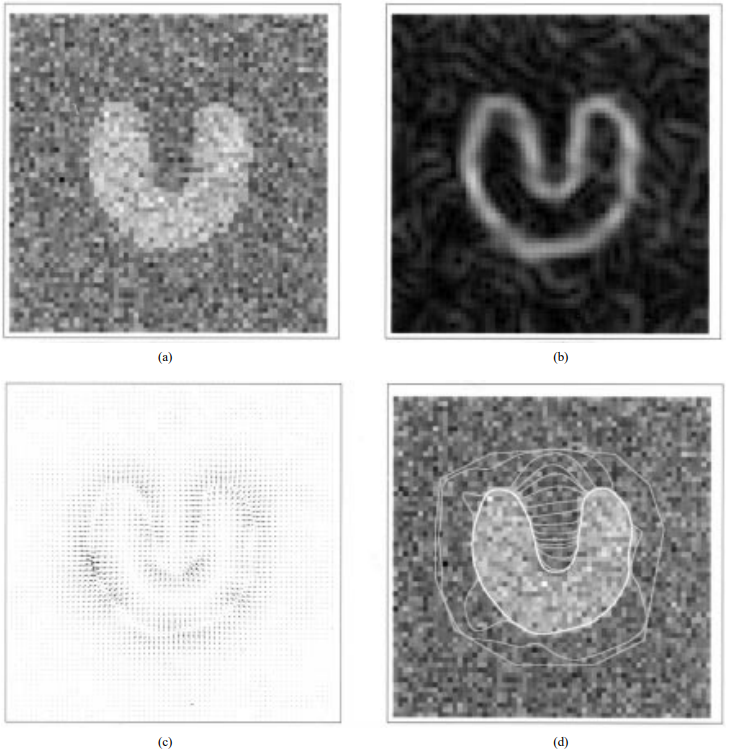
\includegraphics[width=1\textwidth]{gambar/gvfilu}
	\caption{(a) citra objek U yang memiliki \emph{noise}; (b) \emph{edge map}; (c) medan gaya eksternal GVF; dan (d) konvergensi GVF \emph{snake} \citep{xu1998snakes:22}.}
	\label{Gambar:gvfilu}
\end{figure}


% Baris ini digunakan untuk membantu dalam melakukan sitasi
% Karena diapit dengan comment, maka baris ini akan diabaikan
% oleh compiler LaTeX.
\begin{comment}
bibliography{daftar-pustaka}
\end{comment}
